\stepcounter{chapter}
\chapter{First time}
    
    \begin{problem}[Seconds]\label{problem_2.1}
        For this problem we have to
        \begin{enumerate}
            \item Write a script that calculates the number of seconds, $s$, given the number of hours, $h$, according to the formula $s=3600$ $h$
            \item Use the script to find the number of seconds in $1.5$, $12$ and $24$ $h$
        \end{enumerate}
    \end{problem}
    \textit{ Sol. } 
    \lstinputlisting[language=Python]{Programs/chapter2/2_1_seconds.py}
    \begin{verbatim}
        1.5 hours is equivalent 5400.0 seconds
        12.0 hours is equivalent 43200.0 seconds
        24.0 hours is equivalent 86400.0 seconds
    \end{verbatim}


    \begin{problem}[Spherical mass]\label{problem_2.2}
        For this problem we have to
        \begin{enumerate}
            \item Write a script that calculates the mass of a sphere given its radius $r$ and mass density $\rho$ according to the formula $m=\qty(4\pi/3)\rho r^{3}$.
            \item Use the script to find the mass of a sphere of steel of radius $r=1$ mm, $r=1$ m and $r=10$ m.
        \end{enumerate}
    \end{problem}
    \textit{ Sol. }
    \lstinputlisting[language=Python]{Programs/chapter2/2_2_Spherical_mass.py}
    \begin{verbatim}
        The sphere of steel with density 8000 kg/m3
        The sphere with 0.001 m of radius has 3.351032163829113e-05 kg
        The sphere with 1.0 m of radius has 33510.32163829113 kg
        The sphere with 10.0 m of radius has 33510321.638291128 kg
    \end{verbatim}

   
    \begin{problem}[Angle]\label{problem_2.3}
        For this place we have to
        \begin{enumerate}
            \item Write a function that for a point $\qty(x,y)$ returns the angle $\theta$ from the $x$-axis using the formula $\theta = \arctan{\qty(y/x)}$.
            \item Find the angles $\theta$ for the points $\qty(1,1)$, $\qty(-1,1)$, $(-1,-1)$, $(1,-1)$.
            \item How would you change the function to return values of $\theta$ in the range $\qty[0,2\pi]$?
        \end{enumerate}
    \end{problem}


    \begin{problem}[Unit vector]\label{problem_2.4}
        For this problem we have to
        \begin{enumerate}
            \item Write a function that returns the two-dimensional unit vector, $\qty(u_x,u_y)$, corresponding to an angle $\theta$ with the $x$-axis. You can use the formula $\qty(u_x,u_y)=\qty(\cos{\theta},\sin{\theta})$, where $\theta$ is given in radians.
            \item Find the unit vectors for $\theta = 0, \pi/6, \pi/3, \pi/2, 3\pi/2$.
            \item Rewrite the function to instead take the argument $\theta$ in degrees.
        \end{enumerate}
    \end{problem}
    \textit{ Sol. } 
    \lstinputlisting[language=Python]{Programs/chapter2/2_4_Angle.py}
    \begin{verbatim}
The unit vectors for 0 radiants are (1.0, 0.0)
The unit vectors for 0.5235987755982988 radiants are (0.86602540378, 0.49999999999)
The unit vectors for 1.0471975511965976 radiants are (0.50000000000, 0.86602540378)
The unit vectors for 1.5707963267948966 radiants are (6.123233995736766e-17, 1.0)
The unit vectors for 4.71238898038469 radiants are (-1.8369701987210297e-16, -1.0)
    \end{verbatim}


    \begin{problem}[Plotting the normal distribution]\label{problem_2.5}
        The normal distribution, often called the Gaussian distribution, is given as:
        \begin{equation} \label{eqt = normal_distribution}
            P\qty(x;\mu,\sigma) = \frac{1}{\sqrt{2\pi\sigma^{2}}} e^{-\qty(x-\mu)^{2} / \qty(2\sigma)^2}
        \end{equation}
        Where $mu$ is the average and $sigma$ is the standard deviation.
        \begin{enumerate}
            \item Make a function \verb|normal(x,mu,sigma)| that returns the normal distribution value $P\qty(x,\mu,\sigma)$ as given by the formula \ref{eqt = normal_distribution}.
            \item Use this function to plot the normal distribution for $-5<x<5$ for $\mu=0$ and $\sigma=1$.
            \item Plot the normal distribution for $-5<x<5$ for $\mu=0$ and $\sigma=2$ and $\sigma=0.5$ in the same plot.
            \item Plot the normal distribution $-5<x<5$ for $\sigma=1$ and $\mu=0,1,2$ in three subplots above each other.
        \end{enumerate}
    \end{problem}
    \textit{ Sol. }
    \lstinputlisting[language=Python]{Programs/chapter2/2_5__Plotting_normal.py}
    \begin{figure}[h!]
        \centering
        \begin{subfigure}[b]{0.4\linewidth}
            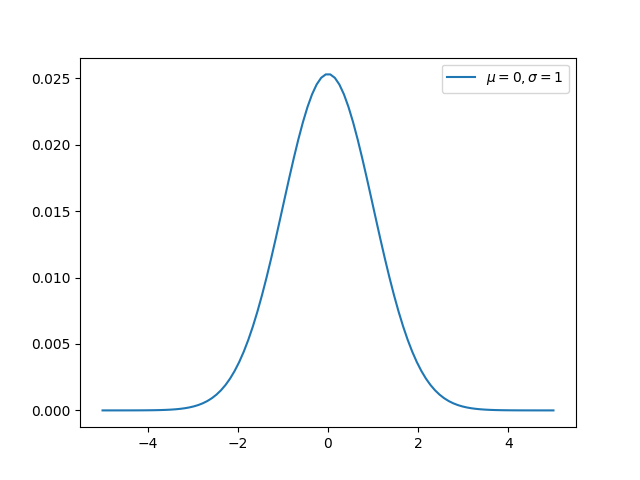
\includegraphics[width=\linewidth]{img/chapter2/2-5/2_5_plot_a.png}
            \caption{For $-5<x<5, \ \mu=0$ and $\sigma=1$}
        \end{subfigure}
        \begin{subfigure}[b]{0.4\linewidth}
            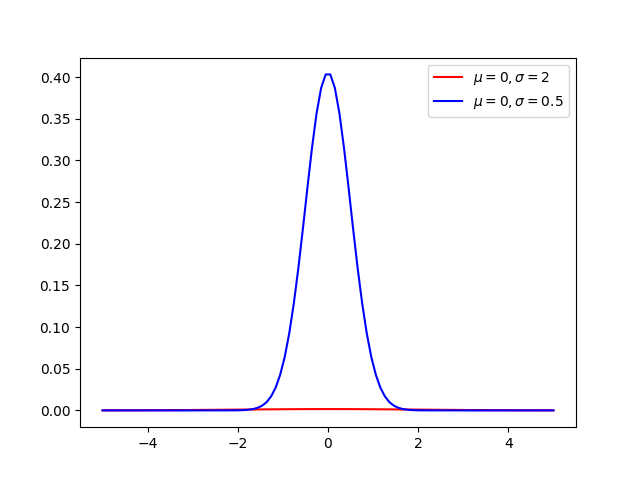
\includegraphics[width=\linewidth]{img/chapter2/2-5/2_5_plot_b.png}
            \caption{For $-5<x<5, \ \mu=0$ and $\sigma=2,0.5$}
        \end{subfigure}
        \begin{subfigure}[b]{0.5\linewidth}
            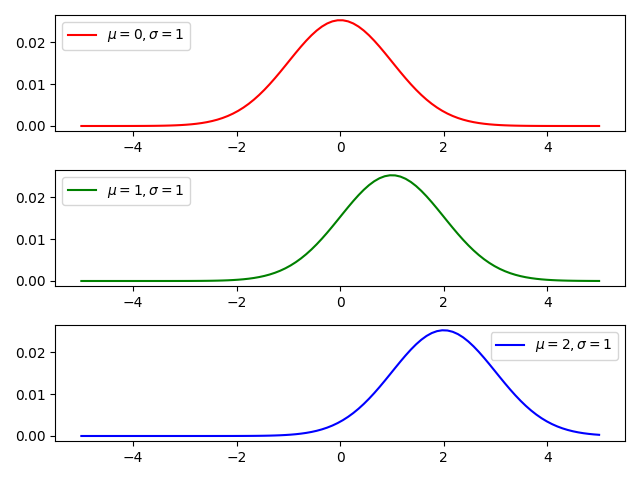
\includegraphics[width=\linewidth]{img/chapter2/2-5/2_5_plot_c.png}
            \caption{For $-5<x<5, \ \mu=0,1,2$ and $\sigma=1$}
        \end{subfigure}
        \caption{Solutions of the problem \ref{problem_2.5}}
        \label{fig:problem 2-5}
    \end{figure}


    \begin{problem}[Plotting $1/x^{n}$]\label{problem_2.6}
        The function $f\qty(x;n)$ is given as $f\qty(x;n)=x^{-n}$
        \begin{enumerate}
            \item Make a function \verb|f(x,n)| which returns the value of $f\qty(x;n)$.
            \item Use this function to plot $1/x$, $1/x^{2}$ and $1/x^{3}$ in the same plot for $-1<x<1$.
        \end{enumerate}
    \end{problem}
    \textit{ Sol. }
    \lstinputlisting[language=Python]{Programs/chapter2/2_6_Plotting_1x_n.py}
    \begin{figure}[h!]
        \centering
        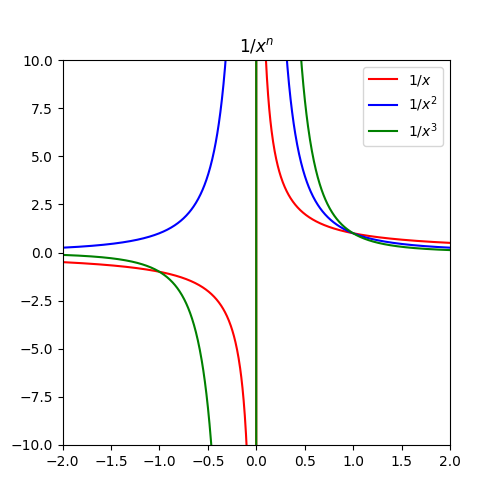
\includegraphics[width=0.5\linewidth]{img/chapter2/2-6/2_6_plot_xs.png}
        \caption{Graphs for $n=1,2,3$}
        \label{fig:problem 2-6} 
    \end{figure}


    \begin{problem}[Plotting $\sin{x}/x^{n}$]\label{problem_2.7}
        The function $g\qty{x;n}$ is given as:
        \begin{equation}\label{eqt = sin_x_over_xn}
            g\qty(x;n) = \frac{\sin{x}}{x^{n}} 
        \end{equation}
        \begin{enumerate}
            \item Make a function \verb|gvalue(x,n)| which returns the value of $g\qty(x;n)$.
            \item Use this function to plot $\sin{x}/x$, $\sin{x}/x^{2}$ and $\sin{x}/x^{3}$ in the same plot for $-5<x<5$.
            \item Use the help function to find out how to place legends for each of the plots into the figure.
        \end{enumerate}
    \end{problem}
    \textit{ Sol. }
    \lstinputlisting[language=Python]{Programs/chapter2/2_7_Plotting_sinx.py}
    \begin{figure}[h!]
        \centering
        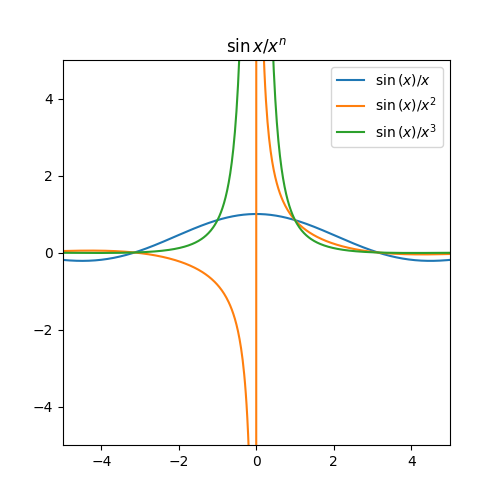
\includegraphics[width=0.5\linewidth]{img/chapter2/2-7/2_7_plot_sinx.png}
        \caption{Graphs for $n=1,2,3$}
        \label{fig:problem 2-7}
    \end{figure}


    \begin{problem}[Logistic map]\label{problem_2.8}
        The iterative mapping $x\qty(i+1)=rx\qty(i) \qty(1-x\qty(i))$ is called the logistic map.
        \begin{enumerate}
            \item Make a function \verb|logistic(x,r)| which returns the value of $x\qty(i+1)$ given $x\qty(i)$ and $r$ as inputs.
            \item Write a script with a loop to calculate the first 100 steps of the logistic map starting from $x\qty(1)=0.5$. Store all the values in an array \verb|x| with $n=100$ elements and plot $x$ as a function of the number of steps $i$:
            \item Explore the logstic map for $r=1.0, \ 2.0, \ 3.0$ and $4.0$
        \end{enumerate}
    \end{problem}
    \textit{ Sol. }
    \lstinputlisting[language=Python]{Programs/chapter2/2_8_logistic_map.py}
    \begin{figure}[h!]
        \centering
        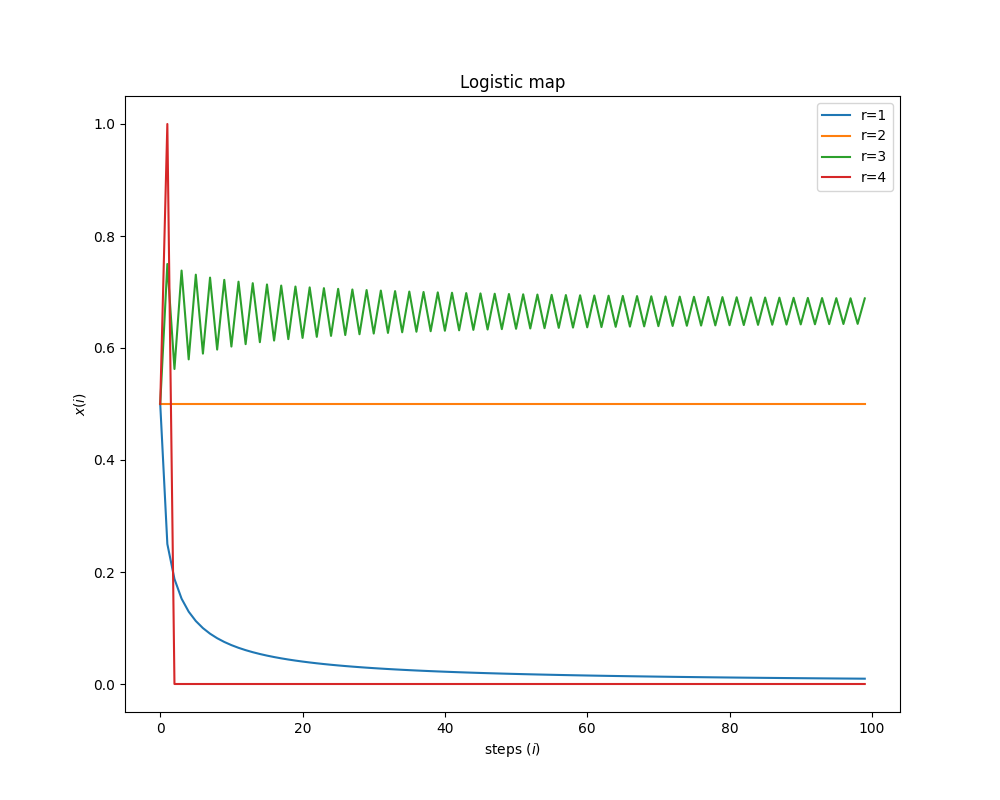
\includegraphics[width=0.85\linewidth]{img/chapter2/2-8/2_8_logistic_map.png}
        \caption{Graphs for $r=1,2,3,4$ and $x(1)=0.5$}
        \label{fig:problem 2-8}
    \end{figure}
    

    \begin{problem}[Euler's Method]\label{problem_2.9}
        In mechanics, we often use Euler's method to determine the motion of an object given how the acceleration depends on the velocity and position of an object. For example, we may know that the acceleration $a(x, v)$ is given as $a\qty(x, v) = - kx - cv$. If we know the position $x$ and the velocity $v$ at a time $t = 0$: $x(0) = x_0 = 0$ and $v(0) = v_0 = 1$, we can use Euler's method to find the position and velocity after a small timestep $\Delta t$:
        \begin{align}
            v_{i} = v\qty(t_{i-1} + \Delta t) & = v\qty(t_{i-1}) + a\qty(v\qty(t_{i-1}),x\qty(x_{0})) \Delta t \\
            x_{i} = x\qty(t_{i-1} + \Delta t) & = x\qty(t_{i-1}) + v\qty(t_{i-1}) \Delta t 
        \end{align}
        and so on. We can therefore use this scheme to find the position x(t) and the velocity $v(t)$ as function of time at the discrete values $t_{i} = i\Delta t$ in time.
        \begin{enumerate}
            \item Write a function \verb|acceleration(v,x,k,C)| which returns the value of $a\qty(x,v)=-kx-Cv$.
            \item Write a script that calculates the first 100 values of $x(t_{i})$ and $v(t_{i})$ when $k=10$, $C=5$ and $\Delta t =0.01$. Plot $x(t)$, $v(t)$ and $a(t)$ as functions of time.
            \item What would you need to change to instead find $x(t)$ and $v(t)$ is the acceleration was given as $a\qty(v,x)=k\sin{x}-Cv$?
        \end{enumerate}
    \end{problem}
    \textit{ Sol. }
    \lstinputlisting[language=Python]{Programs/chapter2/2_9_Euler_me.py}
    \begin{figure}[h!]
        \centering
        \begin{subfigure}[b]{\linewidth}
            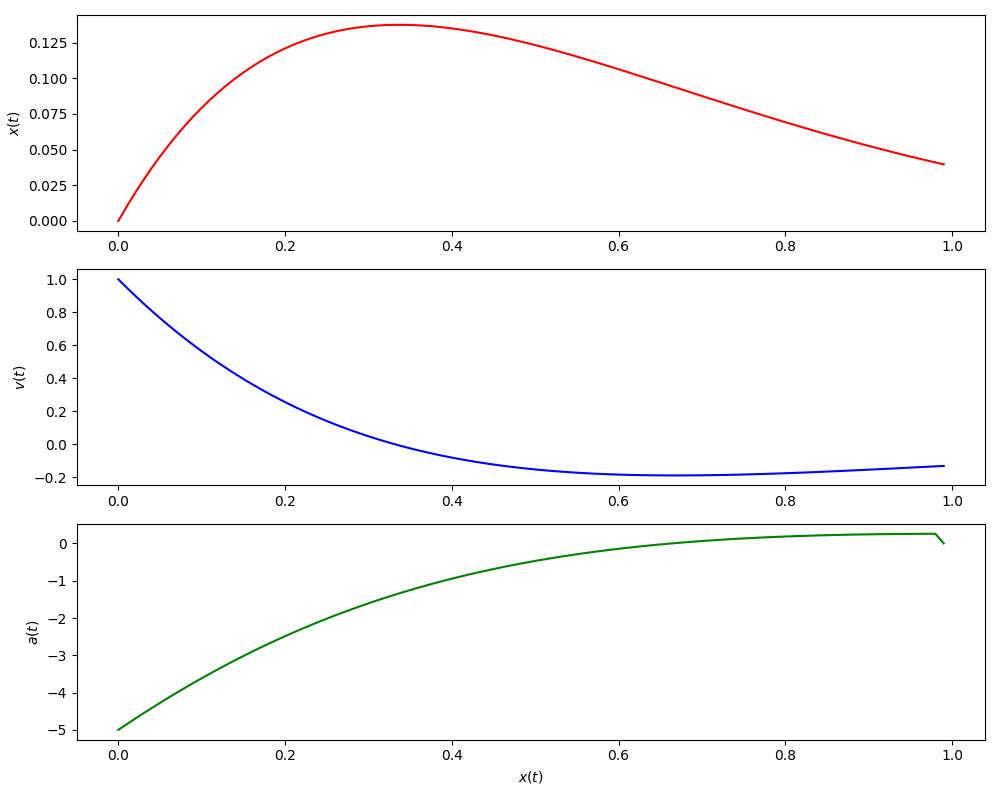
\includegraphics[width=0.9\linewidth]{img/chapter2/2-9/2_9_accele_a.png}
            \caption{Graph for $a(x,v) = -kx-Cv$}
        \end{subfigure}
        \begin{subfigure}[b]{\linewidth}
            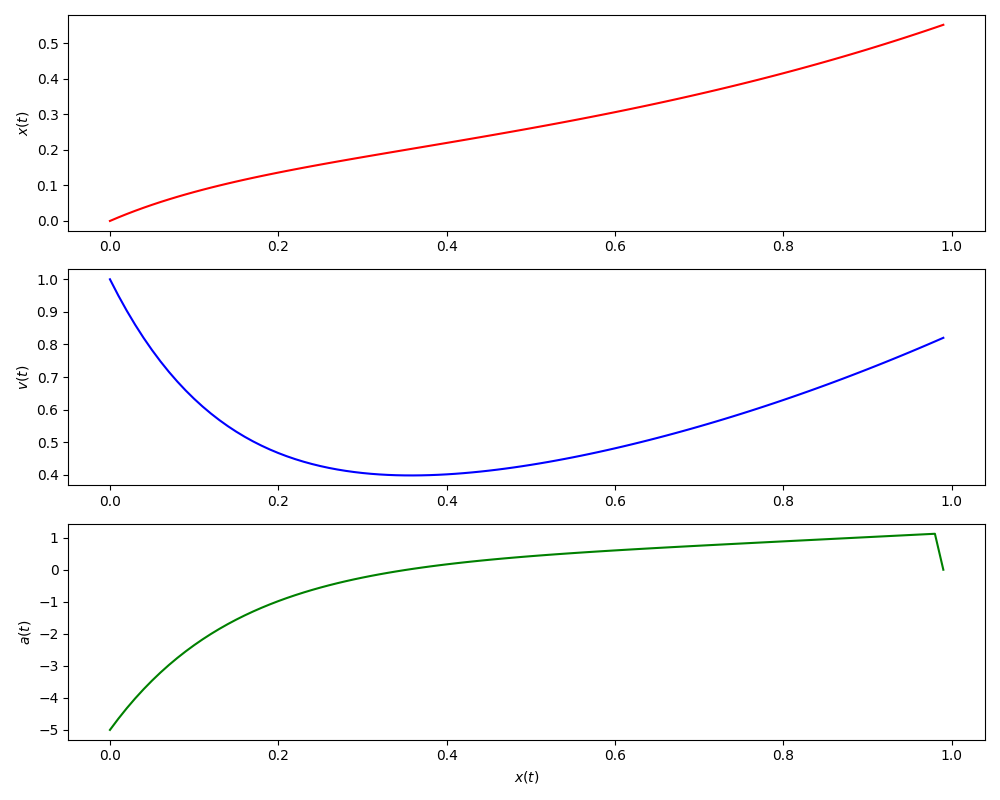
\includegraphics[width=0.9\linewidth]{img/chapter2/2-9/2_9_accele_b.png}
            \caption{Graph for $a(x,v) = k\sin{x}-Cv$}
        \end{subfigure}
        \caption{Solutions of the problem \ref{problem_2.9}}
        \label{fig:problem 2-9}
    \end{figure}